\documentclass{article}
\usepackage{graphicx} % takes care of graphic including machinery
\usepackage{geometry} % decreases margins
\usepackage{amsmath}
\usepackage{cite}
\usepackage[final]{hyperref}
\usepackage{amsfonts}
\usepackage{ctable}
\hypersetup{
	colorlinks=true,       % false: boxed links; true: colored links
	linkcolor=blue,        % color of internal links
	citecolor=blue,        % color of links to bibliography
	filecolor=magenta,     % color of file links
	urlcolor=blue         
}

%++++++++++++++++++++++++++++++++++++++++

\parindent = 0 pt
\begin{document}

\title{Exam Problem 11}
\author{Andreas Nygaard}
\date{\today}
\maketitle

\section*{Problem Description}

\begin{center}
\textbf{Multidimensional pseudo-random (plain Monte Carlo) vs quasi-random (Halton and/or lattice sequence) 
integrators}
\vspace{0.4cm}

\textit{Investigate the convergence rates (of some interesting integrals in different dimensions) as function 
of the number of sample points.}
\end{center}


\section*{Solution}

I have implemented two sequences for quasi-random Monte Carlo integration, which is the Lattice sequence
and the Halton sequence. These low-discrepancy sequences should converge faster than the pseudo-random
Monte Carlo integration, since we make sure that the sampling points are more evenly distributed. Because
the sampling points of the pseudo-random method are statistically independent, we have a finite probability
of all sampling points ending up in only one half of the integration region. This independency is eliminated
in the quasi-random case, which ensures a faster convergence\cite{ppnm}. The convergence rate (the decrease of error) of 
the pseudo-random method is $\mathcal{O}(1/\sqrt{N})$, where $N$ is the number of sampling points, and the 
convergence rate of the quasi-random method is close to $\mathcal{O}(1/N)$. For an integral of dimension $s$
we can put an upper limit on the convergence rate at $\mathcal{O}(\log(N)^s/N)$, which means that the error
will at least decrease as fast as this\cite{wiki}. We will see that it actually converges faster than this upper bound,
but not quite as fast as the $\mathcal{O}(1/N)$ estimate either.
\\

Using 5000 sampling points, I have calculated the integral of the Himmelblau's function, $f(x,y)=(x^2+y-11)^2+(x+y^2-7)^2$,
from 0 to 6 in both dimensions, which analytically is

\begin{equation}
	\int_0^6\mathrm{d}x\int_0^6\mathrm{d}y\,(x^2+y-11)^2+(x+y^2-7)^2 = 11\,390.4
\end{equation}

In table \ref{tab:int} we see the results of a calculation with these three methods.
The estimated errors of the quasi-random methods are no good, since the
central limit theorem doesn't apply when the points are not statistically
independent\cite{ppnm}. Instead we use the difference in the integral estimates of
the two quasi-random sequences Lattice and Halton as an error estimate in the following treatment.
\\

\begin{table}[t]
\centering
\begin{tabular}{c|ccc}
                        & Pseudo-Random\footnotemark
                                        & Lattice      & Halton       \\ \specialrule{.1em}{.05em}{.05em} 
\textsl{Integral}       & $11\,268.07$  & $11\,296.72$ & $11\,363.40$ \\
\textsl{Exact Error}    & $122.33$      & $93.68$      & $27.00$      \\
\textsl{Error Estimate} & $175.17$      & -            & -           
\end{tabular}
\caption{\textsl{Estimates of the integral of the Himmelblau's function using all three
sampling methods. All of these calculations have $N=5000$.}}
\label{tab:int}
\end{table}


Figure \ref{fig:sample} shows the sampling points of the three methods
when calculating the integral of the Himmelblau's function. The lattice
is very clear in the Lattice sequence, and the Halton sequence gives a
much more evenly distributed sampling than the pseudo-random Monte Carlo.
\\
\footnotetext{Changes each run, so this is an example from a previous run.}

\begin{figure}[t]
    \centering
    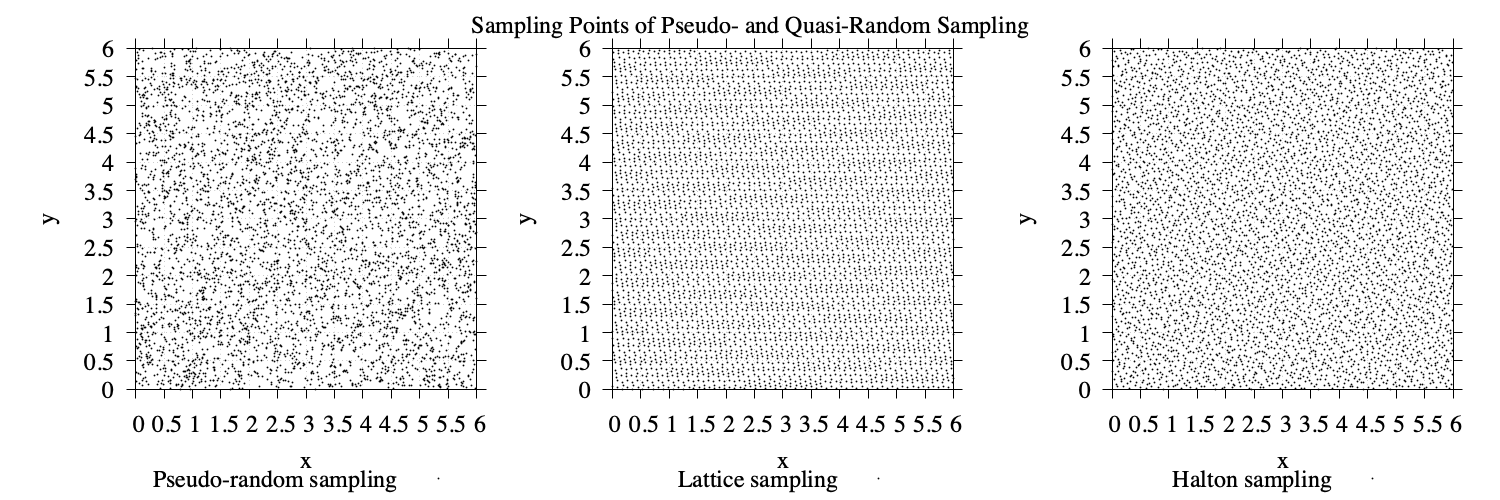
\includegraphics[width=\textwidth]{Sample.png}
    \caption{\textsl{Sampling points of the three methods (Pseudo-random, Lattice sequence and Halton sequence) 
when calculating the integral of the Himmelblau's function. The number of points is $N=5000$ for all three 
methods.}}
    \label{fig:sample}
\end{figure}

We will test error as a function of number of sampling points, $N$, (convergence rate) using integrals
of three different dimensions - 1D, 2D and 5D. 
\\

We start with a 1D integral:
\begin{equation}
        \int_0^{\pi} \mathrm{d}x\, x^3\exp(-x^2) = 
\frac{1}{2}-\frac{1}{2}\exp(-\pi^2)(1+\pi^2)\approx0.49972
\end{equation}
The result of this is seen in figure \ref{fig:1D}, where we show both the estimated and
actual error of both the pseudo-random and quasi-random method. The actual error of the
quasi-random method is measured from the estimated integral of the Lattice sequence method,
while the estimated error is the difference between the estimated integrals of Lattice and
Halton as mentioned previously. The figure also shows the $\mathcal{O}(1/\sqrt{N})$ behavior
separately along with $\mathcal{O}(\log(N)^s/N)$ behaviors for $s=0,1$.
\\

We will use the Himmelblau's function to test the error in 2D. We integrate from 0 to 6
in both dimensions. The result of this is seen in figure \ref{fig:2D}, 
where we show the same as before but now with $s=0,1,2$.
\\

We will also check the convergence of a 5D integral from 0 to 2 in alle five dimensons:
\begin{equation}
	\int_{[0,2]^5} \mathrm{d}V f(x,y,z,p,q) = \int_0^2 \mathrm{d}x \int_0^2 \mathrm{d}y \int_0^2 \mathrm{d}z
\int_0^2 \mathrm{d}p \int_0^2 \mathrm{d}q \, x\cdot p^2 -10 z\cdot q + 5y^2 = -64
\end{equation}

The result is seen in figure \ref{fig:5D}, where we show the same as before but now with $s=0,1,2,3,4,5$.
A zoom-in on the figure also shows the behavior of the convergence at relatively small $N$.
\\

\begin{figure}[t]
    \centering
    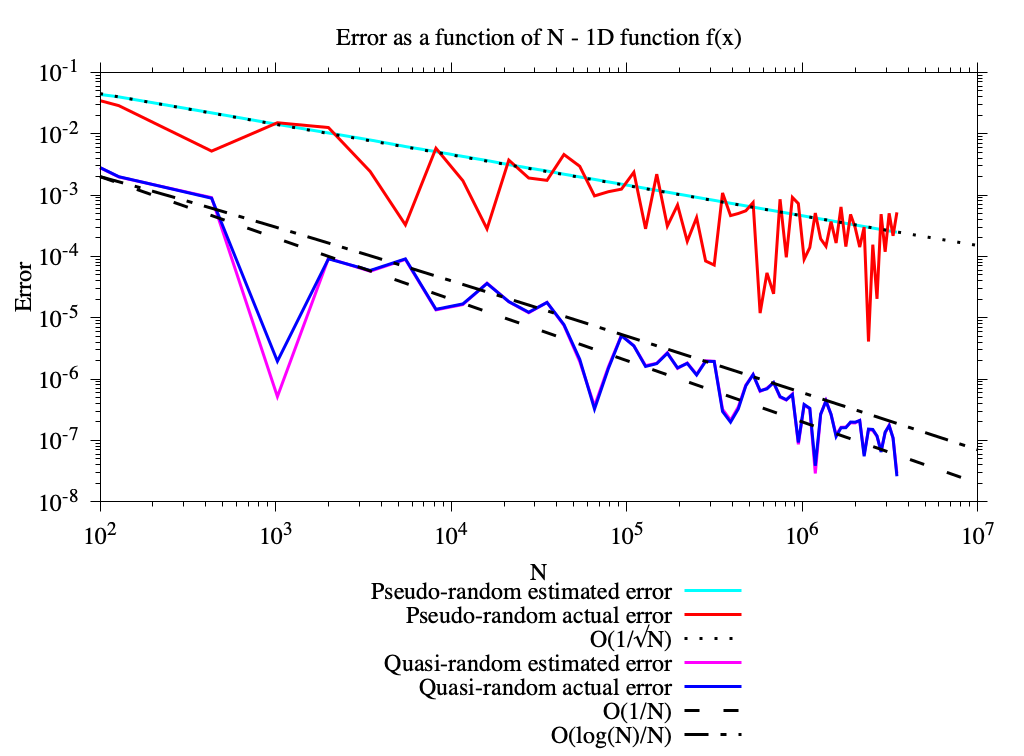
\includegraphics[width=\textwidth]{Convergence1D.png}
    \caption{\textsl{Pseudo- and quasi-random convergence rates for a 1D integral. The integral is that
of the function:} $f(x)=x^3\cdot\exp(-x^2),$ \textsl{from $x=0$ to $x=\pi$.}}
    \label{fig:1D}
\end{figure}

\begin{figure}[t]
    \centering
    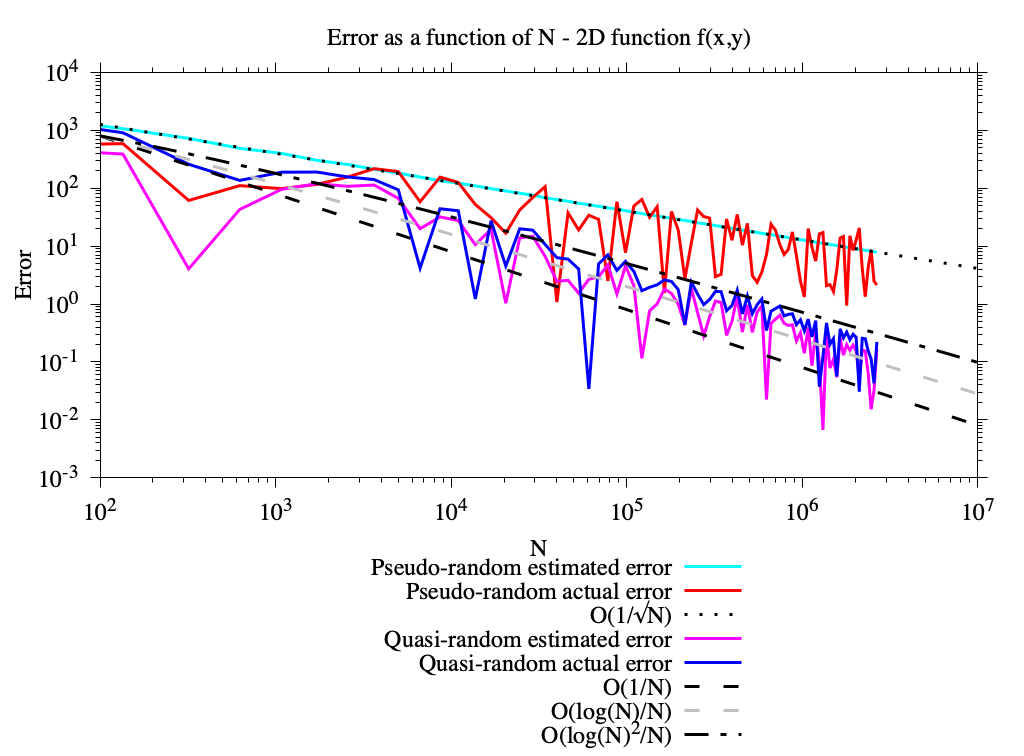
\includegraphics[width=\textwidth]{Convergence2D.png}
    \caption{\textsl{Pseudo- and quasi-random convergence rates for a 2D integral. The integral is that 
of the Himmelblau's function:} $f(x,y)=(x^2+y-11)^2+(x+y^2-7)^2,$ \textsl{from 0 to 6 in both dimensions.}}
    \label{fig:2D}
\end{figure}


\begin{figure}[t]
    \centering
    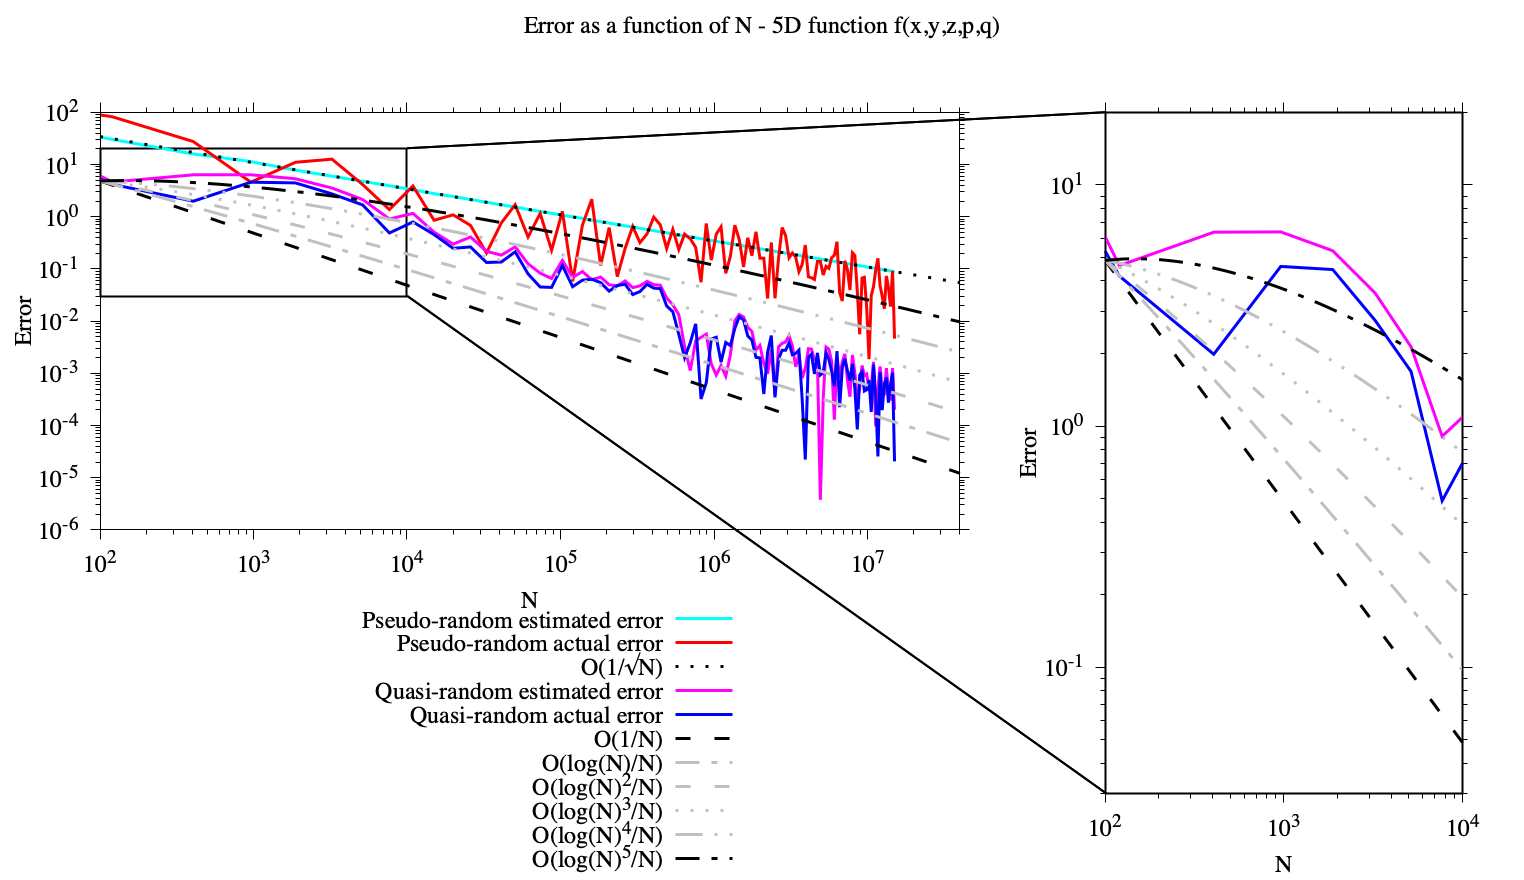
\includegraphics[width=\textwidth]{Convergence5D.png}
    \caption{\textsl{Pseudo- and quasi-random convergence rates for a 5D integral. The integral is that 
of the function:} $f(x,y,z,p,q)=x\cdot p^2 -10 z\cdot q + 5y^2,$ \textsl{from 0 to 2 in all five dimensions.}}
    \label{fig:5D}
\end{figure}



We clearly see that the error of the quasi-random method falls faster with respect
to $N$ than that of the pseudo-random method which falls as $\mathcal{O}(1/\sqrt{N})$, for all cases (1D, 2D and
5D) - mostly clear for the estimated error but also the actual to some extend. As mentioned before, an upper bound on
the behavior of the quasi-random error estimation should be $\mathcal{O}(\log(N)^s/N)$, where $s$ is the dimension. In the
1D case, it is not clear exactly which behavior the quasi-random error exhibits, but it seems to fall between the
$\mathcal{O}(\log(N)/N)$ (upper bound for $s=1$) and $\mathcal{O}(1/N)$. In the
2D case, it is not clear from the figure whether the quasi-random error falls as
$\mathcal{O}(\log(N)^2/N)$ or as $\mathcal{O}(\log(N)/N)$, but we can however see that it doesn't fall slower
than $\mathcal{O}(\log(N)^2/N)$ and it doesn't fall as fast as just $\mathcal{O}(1/N)$.
When examining the 5D case, we see that the $\mathcal{O}(\log(N)^5/N)$ behavior might hold for
smaller $N$ (still large enough to give a reasonable result though), but for very
large $N$ it seems to fall down to an $\mathcal{O}(\log(N)^2/N)$ behavior or at least faster than
the upper bound. We can once again think of the $\mathcal{O}(1/N)$ behavior as a lower bound,
which brings the conclusion:
\\

\textbf{For quasi-random methods, the error as a function of $N$ falls somewhere between the
behaviors $\mathcal{O}(1/N)$ (lower bound) and $\mathcal{O}(\log(N)^s/N)$ (upper bound) where $s$ is the 
dimension, thus making it faster converging than the pseudo-random method with
convergence rate $\mathcal{O}(1/\sqrt{N})$.}


%+++++++++++++++++++++++++++++++++++++++
\newpage
\begin{thebibliography}{99}

\bibitem{ppnm} D. V. Federov, \emph{Monte Carlo integration},  available at
\url{http://62.107.14.89/~fedorov/prog/book/montecarlo.pdf}.

\bibitem{wiki} \emph{Quasi-Monte Carlo method},  available at
\url{http://en.wikipedia.org/wiki/Quasi-Monte_Carlo_method}.

\end{thebibliography}


\end{document}

